% Teorijski deo zasnovan na:
% Richard Szeliski, Computer Vision: Algorithms and Applications, 2010 draft.
% U tvojoj literaturi ovo je referenca [1].
%
% Predlog: ovaj fajl ubaciti umesto/sadržajno proširiti postojeće poglavlje
% "OSNOVE KOMPJUTERSKE VIZIJE ZA ANALIZU HODA".
%
% Slike iz ovog paketa su isečene iz PDF-a koji si priložio. U radu ih obavezno
% navedi kao preuzete/adaptirane iz [1], uz originalni broj slike i stranu.

\chapter{OSNOVE KOMPJUTERSKE VIZIJE ZA ANALIZU HODA}

Kod procene hoda iz video snimka nije dovoljna samo informacija iz jednog frejma. Položaj noge ili trupa u jednom trenutku može da izgleda sasvim normalno, dok se nepravilnost vidi tek kada se posmatra promena kroz vreme. Zbog toga se u ovom radu video posmatra kao niz slika između kojih treba proceniti kretanje. Szeliski probleme ovog tipa razmatra kroz poravnanje slika, parametarske modele kretanja, optički tok i naučene modele kretanja [1]. Ovakva podela je direktno primenljiva i na hod, jer je cilj prvo opisati kretanje, a tek zatim iz tog opisa proceniti kvalitet.

\section{Poravnanje slika i procena translacije}

Najjednostavniji oblik procene kretanja je translaciono poravnanje dve slike. Pretpostavlja se da se sadržaj iz prve slike nalazi u drugoj slici pomeren za vektor $\mathbf{u}=(u,v)$. Za dati pomeraj može se meriti suma kvadrata razlika odgovarajućih piksela, odnosno SSD kriterijum [1, Sec. 8.1]:

\begin{equation}
E_{\mathrm{SSD}}(\mathbf{u})=
\sum_i \left[I_1(\mathbf{x}_i+\mathbf{u})-I_0(\mathbf{x}_i)\right]^2.
\label{eq:ssd_alignment}
\end{equation}

Ovde je $I_0$ prvi frejm, $I_1$ sledeći frejm, $\mathbf{x}_i$ pozicija piksela, a $\mathbf{u}$ procenjeni pomeraj. Razlika

\begin{equation}
e_i=I_1(\mathbf{x}_i+\mathbf{u})-I_0(\mathbf{x}_i)
\end{equation}

predstavlja rezidualnu grešku. Osnovna pretpostavka je da odgovarajuće tačke između dva bliska frejma zadržavaju približno isti intenzitet. Szeliski ovu pretpostavku navodi kao \textit{brightness constancy} [1, p. 384]. Naravno, u realnom videu ona nije savršena. Promena osvetljenja, blur, senke ili refleksije mogu promeniti vrednost piksela i bez fizičkog pomeranja objekta.

Kod humanoidnog hoda ovo je važno jer se ceo robot pomera kroz kadar. Ako se posmatra samo sirovi optički tok, veliki deo vektora predstavlja zajedničko globalno pomeranje tela, a ne relativno kretanje nogu. Zbog toga se u praktičnom delu koristi i body-centered residual flow, gde se dominantna translaciona komponenta proceni i ukloni pre formiranja završnih osobina.

Za veća pomeranja direktna pretraga na punoj rezoluciji postaje skupa i može biti nepouzdana. Szeliski zato opisuje hijerarhijski \textit{coarse-to-fine} pristup [1, Sec. 8.1.1]. Slika se prvo smanjuje u piramidi, pomeraj se proceni na grubom nivou, a zatim se ta procena prenosi na finiji nivo. Za prelaz na sledeći finiji nivo procena pomeraja se približno skalira kao

\begin{equation}
\hat{\mathbf{u}}^{(l-1)} \leftarrow 2\mathbf{u}^{(l)}.
\label{eq:coarse_to_fine}
\end{equation}

Ovo omogućava da se veliki pokreti prvo vide kao manji pokreti na nižoj rezoluciji, posle čega se rezultat postepeno precizira.

\begin{figure}[H]
  \centering
  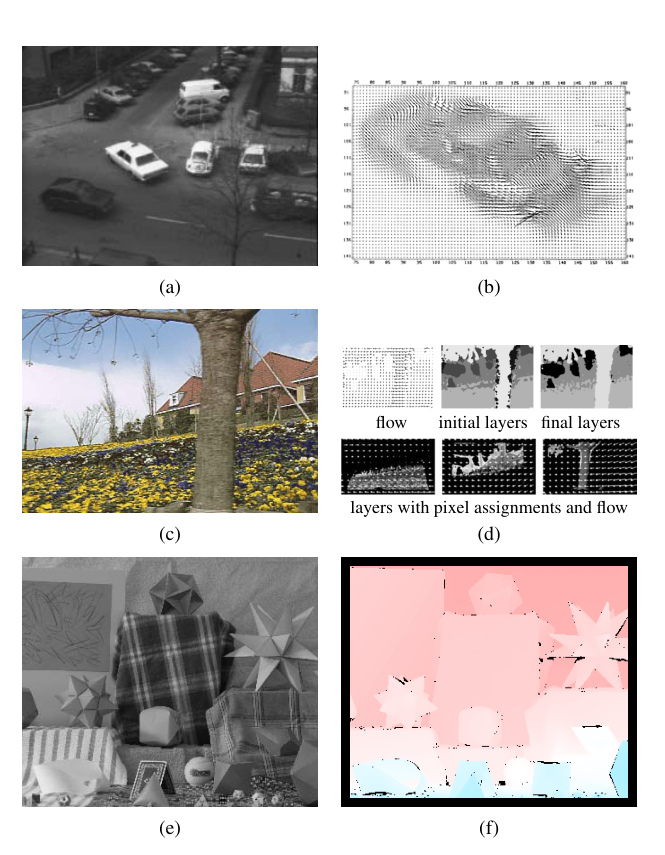
\includegraphics[width=0.78\textwidth]{assets/book_theory/figure_8_1_motion_estimation.png}
  \caption{Primeri procene kretanja i optičkog toka. Preuzeto iz [1], Slika 8.1, str. 382.}
  \label{fig:szeliski_motion_estimation}
\end{figure}

\section{Optički tok}

Optički tok predstavlja procenu prividnog pomeranja u ravni slike. Za razliku od jedne globalne translacije, kod gustog optičkog toka procenjuje se poseban vektor pomeranja za veliki broj piksela, praktično za ceo kadar. Szeliski opšti SSD oblik za optički tok piše kao [1, Sec. 8.4]

\begin{equation}
E_{\mathrm{OF}}(\{\mathbf{u}_i\})=
\sum_i \left[I_1(\mathbf{x}_i+\mathbf{u}_i)-I_0(\mathbf{x}_i)\right]^2.
\label{eq:optical_flow_ssd}
\end{equation}

Ovde svaki piksel ima svoj pomeraj $\mathbf{u}_i$. To odmah pravi problem, jer broj nepoznatih veličina postaje veoma veliki. Zbog toga se lokalne metode oslanjaju na prozore i pretpostavku da susedni pikseli imaju slično kretanje, dok globalne metode dodaju uslov glatkoće polja kretanja.

\subsection{Linearizacija i brightness constancy jednačina}

Za male promene pomeraja može se koristiti Taylorov razvoj intenziteta slike. Lucas--Kanade pristup linearizuje funkciju slike oko trenutne procene pomeraja [1, Sec. 8.1.3; 11]. Na taj način se dobija poznata jednačina optičkog toka

\begin{equation}
I_x u + I_y v + I_t = 0,
\label{eq:brightness_constancy}
\end{equation}

gde su $I_x$ i $I_y$ prostorni izvodi intenziteta, $I_t$ vremenski izvod, a $u$ i $v$ horizontalna i vertikalna komponenta brzine odnosno pomeraja. Jednačina pokazuje da se promena intenziteta može povezati sa kretanjem kroz gradijent slike. Međutim, jedna jednačina nije dovoljna da jednoznačno odredi dve komponente kretanja. Zato se koriste dodatne pretpostavke i informacije iz okoline piksela.

\begin{figure}[H]
  \centering
  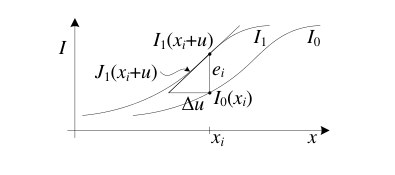
\includegraphics[width=0.58\textwidth]{assets/book_theory/figure_8_2_incremental_flow.png}
  \caption{Taylorova aproksimacija i inkrementalna korekcija optičkog toka. Preuzeto iz [1], Slika 8.2, str. 392.}
  \label{fig:szeliski_incremental_flow}
\end{figure}

Kada se linearizovani problem posmatra u lokalnom prozoru, dobija se sistem normalnih jednačina

\begin{equation}
\mathbf{A}\,\Delta \mathbf{u}=\mathbf{b},
\label{eq:lk_normal}
\end{equation}

pri čemu je

\begin{equation}
\mathbf{A}=\sum_i \mathbf{J}_i^T\mathbf{J}_i,
\qquad
\mathbf{b}=-\sum_i e_i\mathbf{J}_i^T.
\end{equation}

Matrica $\mathbf{A}$ sadrži informaciju o lokalnoj strukturi gradijenata. Ako u regionu nema dovoljno teksture ili postoji samo jaka ivica, sistem može biti loše uslovljen. To je poznati \textit{aperture problem}. U slučaju jedne ivice pouzdano se vidi samo komponenta kretanja normalna na ivicu, dok je komponenta duž ivice neodređena [1, pp. 395--397].

\begin{figure}[H]
  \centering
  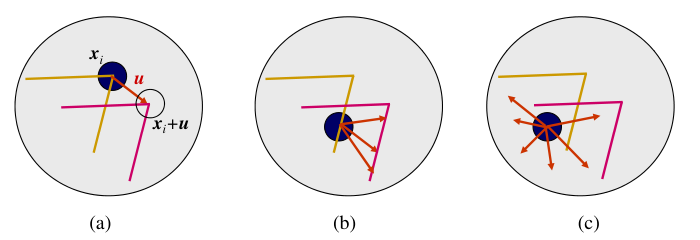
\includegraphics[width=0.85\textwidth]{assets/book_theory/figure_8_3_aperture_problem.png}
  \caption{Aperture problem za teksturisan region, ivicu i region bez teksture. Preuzeto iz [1], Slika 8.3, str. 395.}
  \label{fig:szeliski_aperture}
\end{figure}

Ovo ograničenje je bitno i u našem slučaju. Površine MuJoCo modela mogu biti gotovo jednobojne, pa deo toka na trupu ili ekstremitetima može biti manje pouzdan nego tok na ivicama tela. Zbog toga flow ne treba tumačiti kao direktno i potpuno tačno merenje fizičke brzine robota. On je vizuelna reprezentacija kretanja iz koje se dalje izvlače osobine.

\subsection{Regularizacija optičkog toka}

Szeliski prikazuje i globalni pristup gde se brightness constancy greška posmatra preko cele slike. Ovakav pristup je klasično povezan sa Horn--Schunck formulacijom optičkog toka [12]. Za linearizovani slučaj data-term može da se napiše kao [1, Eq. 8.70]

\begin{equation}
E_{\mathrm{data}}=
\int \left(I_xu+I_yv+I_t\right)^2\,dx\,dy.
\label{eq:flow_data_term}
\end{equation}

Sam data-term nije dovoljan jer je problem optičkog toka potodređen. Zato se dodaje penal koji favorizuje glatko rešenje. U opštem obliku regularizacije iz knjige [1, Sec. 3.7.1] ciljna funkcija je

\begin{equation}
E=E_d+\lambda E_s,
\label{eq:regularization_general}
\end{equation}

gde $E_d$ meri slaganje sa podacima, $E_s$ meri neželjenu neregularnost ili neglatkost, a $\lambda$ određuje odnos ova dva zahteva. Kod toka se ovakva ideja koristi da susedne procene ne menjaju smer i intenzitet potpuno proizvoljno. Sa druge strane, prejaka regularizacija može da izravna stvarne diskontinuitete kretanja, na primer granicu između noge i pozadine.

\section{Naučeni modeli kretanja}

Sirovo polje optičkog toka je veoma visoke dimenzionalnosti. Za svaki frejm postoje horizontalna i vertikalna komponenta na velikom broju piksela. Ako se takva polja koriste direktno, broj karakteristika brzo postaje mnogo veći od broja dostupnih označenih klipova. Zato je korisno pronaći manji broj dominantnih obrazaca kretanja.

Szeliski u odeljku \textit{Learned motion models} opisuje upravo ovakav postupak. Iz trening video sekvenci se prvo računaju gusta polja kretanja, zatim se polja slažu u skup i nad njima se radi singularna dekompozicija. Dobijeni singularni vektori predstavljaju bazna polja kretanja, a novo polje se opisuje njihovom linearnom kombinacijom [1, Sec. 8.2.2; 13]:

\begin{equation}
\mathbf{u}(\mathbf{x})=\sum_k a_k\mathbf{v}_k(\mathbf{x}).
\label{eq:learned_motion_basis}
\end{equation}

Koeficijenti $a_k$ govore koliko je određeni bazni obrazac prisutan u datom trenutku. Posebno je značajno što je primer u knjizi urađen baš na sekvenci hodanja. Na slici su prikazana bazna flow polja, ali i promena njihovih koeficijenata kroz vreme. To je praktično ista ideja koju koristi klasični pipeline ovog rada, samo se kasnije iz vremenskih nizova koeficijenata računaju dodatne osobine.

\begin{figure}[H]
  \centering
  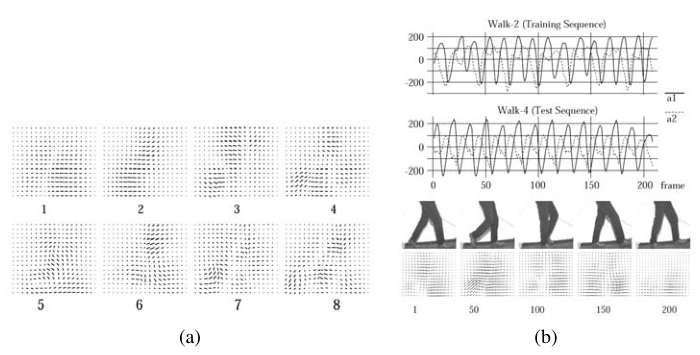
\includegraphics[width=0.90\textwidth]{assets/book_theory/figure_8_6_walking_motion_basis.png}
  \caption{Naučena bazna polja kretanja i vremenski koeficijenti na walking sekvenci. Preuzeto iz [1], Slika 8.6, str. 404.}
  \label{fig:szeliski_walking_basis}
\end{figure}

\section{SVD i PCA redukcija dimenzionalnosti}

Matematička osnova prethodnog postupka je singularna dekompozicija. Za proizvoljnu realnu matricu $\mathbf{A}$ važi [1, App. A.1.1]

\begin{equation}
\mathbf{A}=\mathbf{U}\mathbf{\Sigma}\mathbf{V}^T.
\label{eq:svd}
\end{equation}

Kolone matrica $\mathbf{U}$ i $\mathbf{V}$ su ortonormirani singularni vektori, dok dijagonalna matrica $\mathbf{\Sigma}$ sadrži singularne vrednosti

\begin{equation}
\sigma_0\geq\sigma_1\geq\ldots\geq\sigma_{p-1}\geq 0.
\end{equation}

Ako se zadrži samo prvih $r$ komponenti, dobija se najbolja aproksimacija matrice datog ranga u least-squares smislu [1, Eq. A.5]. To je razlog zbog kojeg mali broj komponenti može da sačuva najveći deo strukture iz velikog vektora optičkog toka.

\begin{figure}[H]
  \centering
  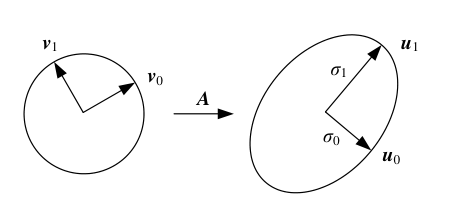
\includegraphics[width=0.58\textwidth]{assets/book_theory/figure_A_1_svd_pca.png}
  \caption{Geometrijsko tumačenje SVD/PCA transformacije. Preuzeto iz [1], Slika A.1, str. 738.}
  \label{fig:szeliski_svd}
\end{figure}

PCA se može formulisti preko kovarijacione matrice [14]. Za skup vektora $\mathbf{x}_i$ sa srednjom vrednošću $\bar{\mathbf{x}}$ kovarijaciona matrica je

\begin{equation}
\mathbf{C}=\frac{1}{n}\sum_i
(\mathbf{x}_i-\bar{\mathbf{x}})(\mathbf{x}_i-\bar{\mathbf{x}})^T.
\label{eq:pca_covariance}
\end{equation}

Svojstveni vektori matrice $\mathbf{C}$ daju glavne pravce varijacije, dok svojstvene vrednosti određuju količinu varijanse duž tih pravaca. Projekcija novog primera na $i$-tu PCA komponentu može da se napiše kao [1, Eq. 14.11]

\begin{equation}
a_i=(\mathbf{x}-\mathbf{m})\cdot\mathbf{u}_i.
\label{eq:pca_projection}
\end{equation}

U ovom radu je bitna i whitening transformacija, jer se ona koristi nad R3D embedding prostorom. Szeliski je zapisuje kao [1, Eq. 14.15]

\begin{equation}
\hat{\mathbf{U}}=\mathbf{U}\mathbf{\Lambda}^{-1/2}.
\label{eq:pca_whitening}
\end{equation}

Intuitivno, običan PCA samo rotira koordinatni sistem u pravce najveće varijanse, dok whitening dodatno skalira komponente prema njihovoj varijansi. Komponente sa vrlo velikom varijansom se smanjuju, a one sa manjom varijansom postaju uporedivije. U radu se ova transformacija fituje isključivo na trening odnosno neoznačenom reprezentacionom skupu, bez korišćenja test politika.

\section{Vremenska struktura i Furijeova analiza}

Hod je približno periodičan proces. Nije uvek potpuno periodičan, posebno kod skretanja ili promene komande, ali se smene oslonca i zamaha nogu ponavljaju. Zbog toga se vremenski nizovi PCA koeficijenata mogu analizirati i u frekvencijskom domenu.

Diskretna Furijeova transformacija signala dužine $N$ u Szeliskom je data kao [1, Eq. 3.54]

\begin{equation}
H(k)=\frac{1}{N}\sum_{x=0}^{N-1}
h(x)e^{-j2\pi kx/N}.
\label{eq:dft}
\end{equation}

Transformacija razdvaja signal na komponente različitih učestanosti. U pravilnom periodičnom hodu veći deo energije može da bude koncentrisan oko dominantne frekvencije koraka i njenih harmonika. Kod nestabilnog ili neregularnog pokreta energija može biti raspoređena šire. Ovo nije samostalna mera kvaliteta, ali predstavlja dodatnu karakteristiku modela.

Szeliski navodi i Parsevalovu teoremu, prema kojoj je ukupna energija signala jednaka energiji njegove Furijeove reprezentacije. Zbog toga je opravdano koristiti spektralnu energiju i odnos energije u različitim frekvencijskim opsezima kao sažete osobine vremenskog signala.

\begin{figure}[H]
  \centering
  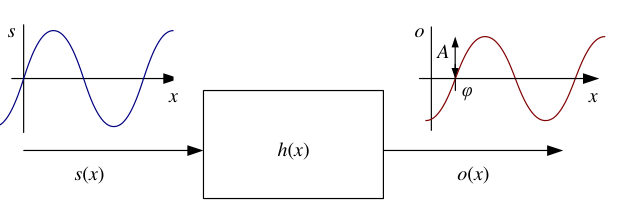
\includegraphics[width=0.78\textwidth]{assets/book_theory/figure_3_24_fourier.png}
  \caption{Osnovna interpretacija Furijeove transformacije preko amplitude i faze sinusoidnog signala. Preuzeto iz [1], Slika 3.24, str. 133.}
  \label{fig:szeliski_fourier}
\end{figure}

\section{Najmanji kvadrati i regularizovana regresija}

Kada se video prevede u konačan vektor osobina, potrebno je proceniti numerički gait score. Knjiga daje opšti oblik linearnog problema najmanjih kvadrata [1, App. A.2]

\begin{equation}
E_{\mathrm{LLS}}=\|\mathbf{A}\mathbf{x}-\mathbf{b}\|^2,
\label{eq:linear_ls}
\end{equation}

čije normalne jednačine imaju oblik

\begin{equation}
(\mathbf{A}^T\mathbf{A})\mathbf{x}=\mathbf{A}^T\mathbf{b}.
\label{eq:normal_equations}
\end{equation}

U praktičnom delu se koristi Ridge regresija, gde se pored greške uvodi i L2 penal nad veličinom koeficijenata. Szeliski ne predstavlja Ridge kao zaseban model u formi u kojoj se koristi u scikit-learn biblioteci, ali teorijska ideja odgovara opštem principu regularizacije iz jednačine~\ref{eq:regularization_general}: model treba da prati podatke, ali se istovremeno kažnjava previše složeno ili nestabilno rešenje. Originalna formulacija Ridge regresije data je u [15].

\section{Veza teorije sa implementacijom}

Klasični deo sistema može se povezati sa prethodnom teorijom u nekoliko koraka. Prvo se video dekodira i frejmovi se vremenski normalizuju. Zatim se procenjuje gusti optički tok. Dominantno globalno pomeranje se umanjuje poravnanjem, posle čega se flow polja svode na manju dimenziju i slažu u matricu. PCA/SVD daje mali broj baznih pravaca kretanja, a koeficijenti tih pravaca se posmatraju kroz vreme. Iz njih se računaju statističke i frekvencijske osobine, koje zatim ulaze u regresioni model.

Ovim se dobijaju dve stvari. Prvo, količina podataka se smanjuje tako da model može da radi i kada postoji mali broj nezavisnih walker politika. Drugo, klasična reprezentacija ostaje dovoljno pregledna da se mogu nacrtati flow polja, bazni pravci i promena koeficijenata kroz vreme. To je razlog zbog kojeg je ovaj pristup zadržan u radu iako je R3D-18 transfer model numerički bolji.

% KRAJ TEORIJSKOG DELA
